\documentclass[conference]{IEEEtran}
\IEEEoverridecommandlockouts
% The preceding line is only needed to identify funding in the first footnote. If that is unneeded, please comment it out.
%Template version as of 6/27/2024

\usepackage{cite}
\usepackage{amsmath,amssymb,amsfonts}
\usepackage{algorithmic}
\usepackage{graphicx}
\usepackage{textcomp}
\usepackage{multirow}
% \usepackage{subcaption} % 支持子图
\usepackage{subfig} 
\usepackage{booktabs} % 需要此宏包来使用 toprule, midrule, bottomrule
\usepackage{amsmath}  % 使用数学符号 (uparrow, downarrow)
\usepackage{xcolor}
\usepackage{xspace}
\usepackage{url}
\usepackage{hyperref}

% \usepackage{xcolor}
% \usepackage[colorlinks=true, urlcolor=black]{hyperref} % 也可以改为 red, green 等颜色



\def\BibTeX{{\rm B\kern-.05em{\sc i\kern-.025em b}\kern-.08em
    T\kern-.1667em\lower.7ex\hbox{E}\kern-.125emX}}

\newcommand{\system}{\textsc{Vulcan}\xspace}

    
\begin{document}

\title{\system: GNN-Enhanced Multi-Agent Cooperative Navigation for Indoor Fire-Disaster Response}

\author{\IEEEauthorblockN{Shengding Liu}
\IEEEauthorblockA{\textit{NetID:} 181595928 \\
\textit{Computer Science \& Engineering} \\
\textit{Michigan State University}\\
East Lansing, MI, USA}
}

\maketitle

\begin{abstract}
Indoor fire disasters pose severe challenges to autonomous search and rescue due to dense smoke, high temperatures, and dynamically evolving environments. In such time-critical scenarios, multi-agent cooperative navigation enables faster and broader exploration than single-agent approaches, but existing systems are predominantly vision-based and designed for benign indoor settings, leading to significant performance degradation under fire-driven conditions. Recent VLM-based planners such as Co-NavGPT inject useful semantic priors but introduce a per-decision latency of $\sim$20\,seconds, a non-trivial API cost, and a hard requirement on network connectivity---all unacceptable for on-board operation in a fire scene where every second compresses the safe operating window. In this paper, we present \system, a multi-modal multi-agent cooperative navigation framework tailored for indoor fire response that retains the original Vulcan stack (multi-modal perception, hazard-aware global mapping, FMM local planner) but replaces the VLM-based global planner with a tiny graph neural network (GNN) student distilled from GPT-4o frontier-assignment decisions. The GNN operates on a bipartite robot--frontier graph, contains fewer than $10^5$ parameters, and runs fully on board. We extend the Habitat-Matterport3D benchmark with physically realistic fire simulations and evaluate \system against the VLM teacher and conventional baselines. On 30 HM3D episodes the GNN matches the VLM's success rate exactly (SR $0.10$ vs.\ $0.10$) while reducing per-decision latency from ${\sim}20{,}000$\,ms to $3.28$\,ms (${\sim}6{,}100\times$ speed-up), removing the API cost, and unlocking high-frequency hazard-aware replanning.
\end{abstract}

\begin{IEEEkeywords}
Search and rescue (SAR), multi-agent systems, cooperative navigation, graph neural networks (GNN), knowledge distillation, vision--language model (VLM), disaster response.
\end{IEEEkeywords}

\section{Introduction}
%\subsection{Background and Motivation}
% the importance of disaster response -> robots replace humans 
Natural and human-made disasters pose immediate threats to life and infrastructure, requiring rapid and coordinated emergency response. In hazardous environments such as indoor fires, high temperature, dense smoke, and structural instability make human intervention extremely dangerous. 
% Whether to put some case studies such as 香港大浦火灾
% As a result, mobile robots have become a promising alternative for operating in life-threatening spaces, providing fast situational awareness, autonomous exploration, and target search capabilities without exposing emergency responders to unnecessary risk.
A recent devastating fire in Tai Po, Hong Kong~\cite{Grundy2025TaiPoFire} greatly impeded human access and situational awareness during the early response phase, leading to significant casualties and property damage. It was the deadliest fire in Hong Kong in decades.

Mobile robots have emerged as a promising alternative for operating in life-threatening environments. By enabling autonomous exploration, hazard perception, and target search under severe perception degradation, robotic systems can provide rapid situational awareness while reducing the risk to human responders and supporting more informed decision-making.

% single robot exploration
Despite recent progress, most existing search and rescue (SAR) deployments~\cite{queralta2008collaborative} still rely on \emph{single-robot exploration} or loosely coordinated multi-robot routines, where individual robots operate with minimal information sharing. Such strategies inherently limit system-level efficiency, particularly in large, unmapped, or dynamically evolving indoor environments, thereby underscoring the urgent need for multi-agent cooperative navigation. 
%To better illustrate the benefits and challenges of multi-agent search and rescue in such hazardous settings, 
Fig.~\ref{fig:scenario} shows an example scenario of multi-agent search and rescue in an indoor fire environment.
% Given that every second is critical in disaster response, these limitations underscore the urgent need for hazard-aware multi-agent collaborative navigation that can reduce exploration latency and improve overall search effectiveness.
% In these settings, inefficient coverage of vast unknown areas, susceptibility to single-robot failures, and delays caused by incorrect decisions or unexpected obstacles can cumulatively degrade mission performance. 
\begin{figure}
    \centering
    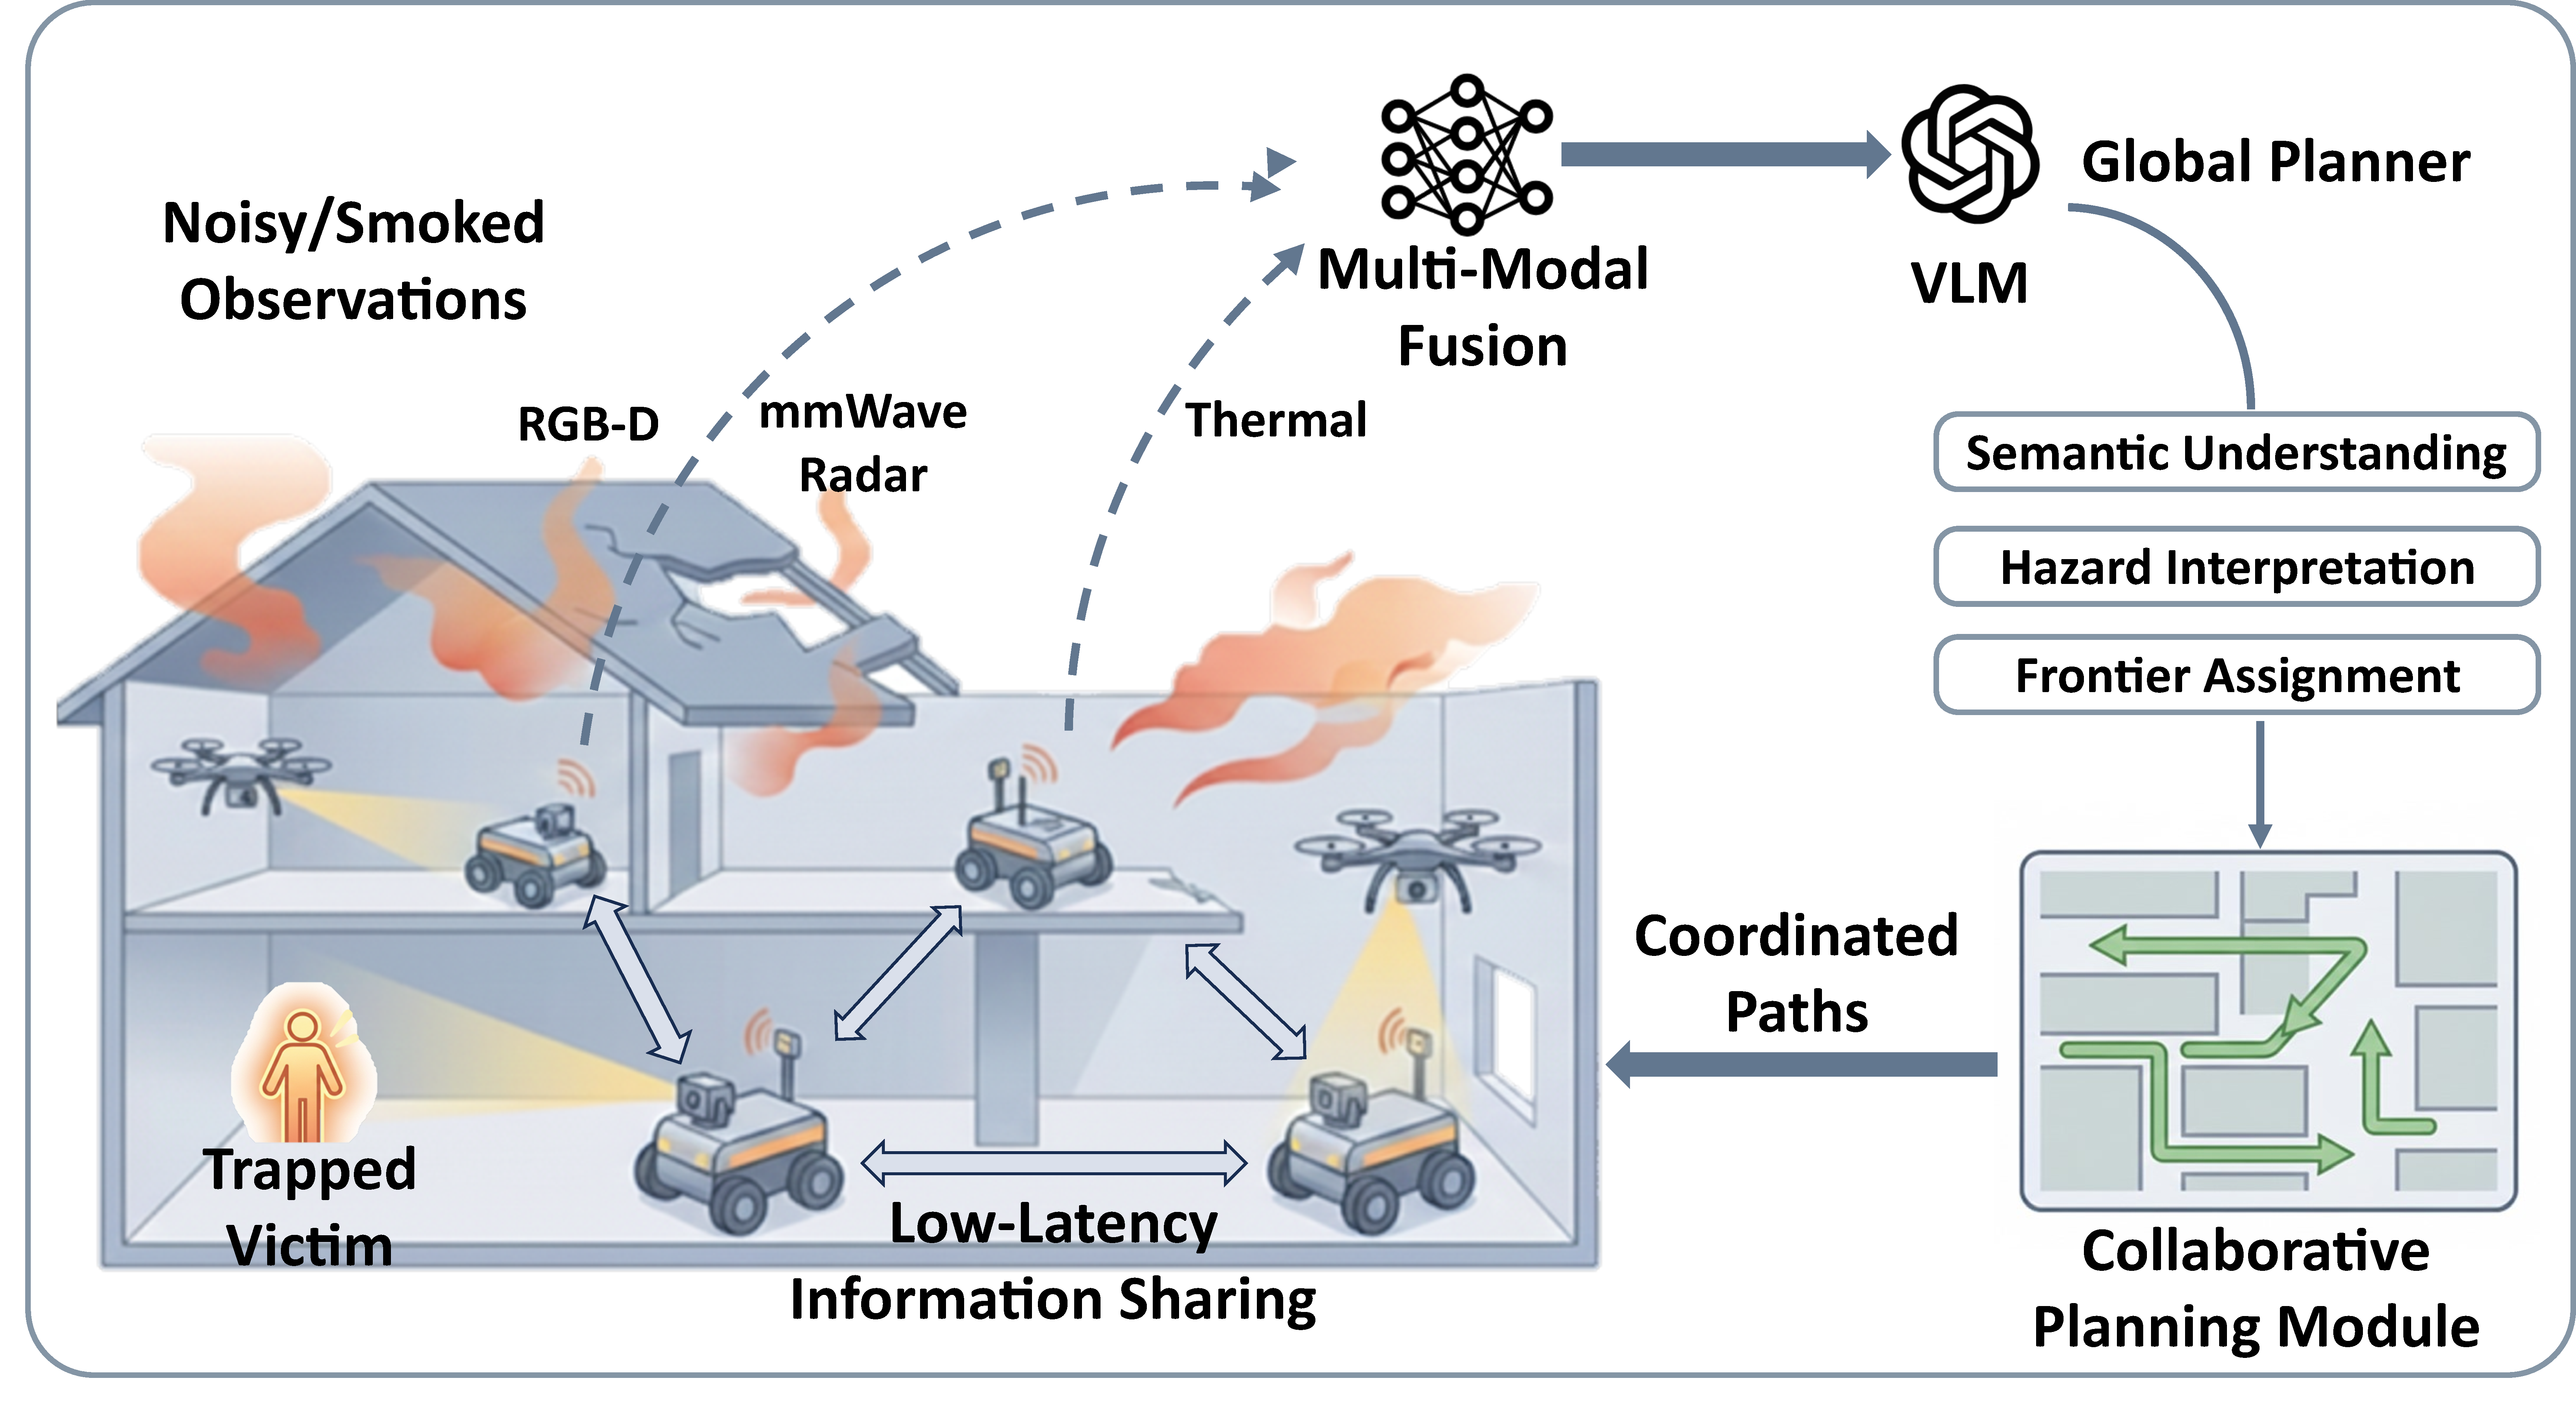
\includegraphics[width=1.0\linewidth]{figures/scenario.pdf}
    \caption{Overview of \system for multi-agent search and rescue in indoor fire scenarios.}%, illustrating sensor observations, multi-modal fusion, VLM-based planning, and coordinated navigation. }
    \label{fig:scenario}
    \vspace{-15pt}
\end{figure}
% 引出视觉导航和VLM导航
\begin{figure}[htbp]
    \centering

    \subfloat[RGB camera]{
        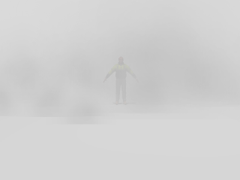
\includegraphics[width=0.45\linewidth]{figures/degradedsensorperformance/rgb.png}
        \label{fig:rgb}
    }
    \hfill
    \subfloat[Depth camera]{
        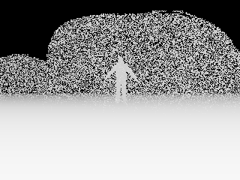
\includegraphics[width=0.45\linewidth]{figures/degradedsensorperformance/depth.png}
        \label{fig:depth}
    }

    %\vspace{0.3cm} % 两行间距，可根据需要调整

    \subfloat[Lidar]{
        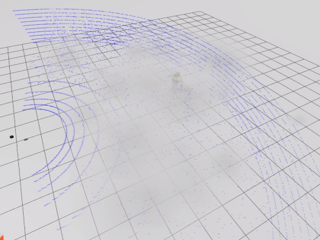
\includegraphics[width=0.45\linewidth]{figures/degradedsensorperformance/lidar.png}
        \label{fig:lidar}
    }
    \hfill
    \subfloat[Thermal camera]{
        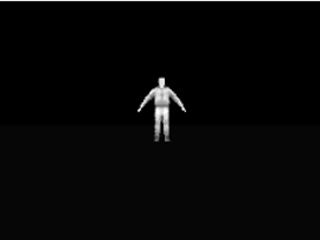
\includegraphics[width=0.45\linewidth]{figures/degradedsensorperformance/thermal.png}
        \label{fig:thermal}
    }

    \caption{Gazebo-based fire simulation demonstrates the degradation of modality-dependent perception  as smoke density increases.}
    \vspace{-15pt}
    \label{fig:four_sensors}
\end{figure}


In recent years, vision-based cooperative navigation has attracted increasing attention, driven by advances in simulation platforms, 
%~\cite{koenig2004design,savva2019habitat}, 
and large-scale 3D scene datasets~\cite{ramakrishnan2021habitat}. Existing approaches to visual navigation are typically grouped into two main paradigms: \emph{end-to-end} systems~\cite{khandelwal2022simple}, which directly map sensory observations to control actions, and \emph{modular pipelines}~\cite{ramakrishnan2022poni}, which explicitly decompose the task into perception, mapping, planning, and control. Both paradigms have demonstrated effectiveness by leveraging spatial and semantic representations learned via supervised or reinforcement learning. Furthermore, recent work has increasingly explored the integration of vision–language
models (VLMs) into visual navigation systems~\cite{11302789}.
%,shen2025enhancing}. 
By jointly reasoning over visual observations and natural language, VLMs introduce powerful semantic priors that enhance object grounding, relational reasoning, and holistic understanding of complex indoor environment. 
%, offering clear performance advantages and emerging as a promising research direction.

However, the majority of existing multi-agent cooperative navigation frameworks~\cite{11302789,liu2024air,yu2022learning} are predominantly vision-based and developed under assumptions of static, well-structured, and relatively benign indoor environments. Such assumptions fundamentally break down in fire-driven indoor scenarios, where perception is severely degraded by smoke and high temperatures, environmental conditions evolve rapidly and unpredictably, and inefficient or uncoordinated exploration can directly compromise both agent safety and mission success. These problems highlight a critical gap in current navigation frameworks and motivate the need for an efficient and safe cooperative multi-agent navigation tailored for indoor fire-disaster response.

\begin{figure*}[t]
  \centering
  \includegraphics[width=\textwidth]{figures/SystemDesign.pdf}
  \caption{System architecture of \system. Each agent performs multi-modal perception and fusion, constructs hazard-aware global maps, and plans safe and efficient exploration using a GNN-based global planner (distilled from a VLM teacher) and a hazard-aware FMM local planner.}
  \label{fig:System Design}
  \vspace{-15pt}
\end{figure*}

%\subsection{Challenges and Contributions}
Despite recent advancements in cooperative navigation including learning-based approaches~\cite{khandelwal2022simple}, VLM powered planning~\cite{11302789}, and embodied multi-agent coordination frameworks~\cite{tan2025roboos}, directly applying these approaches to fire-driven indoor scenarios remains extremely challenging. Compared to static or benign environments, indoor fire scenes introduce several fundamental challenges:

\subsubsection{Dynamic and rapidly evolving environments} 
Temperature gradients, flame propagation, and smoke diffusion continuously reshape the environment, altering traversability, visibility, and semantic cues over time.

\subsubsection{Unreliable and degraded sensor data} 
Fire-induced smoke severely degrades multi-modal perception in indoor environments. 
% Dense smoke scatters and absorbs visible light, significantly impairing RGB-D sensing, while airborne particles directly interfere with LiDAR beams, leading to reduced valid returns as well as spurious measurements such as false echoes and ghost artifacts. In contrast, thermal sensing is comparatively less affected, as it relies on emitted heat rather than optical transparency. 
As illustrated in Fig.~\ref{fig:four_sensors}, our Gazebo-based fire simulations, built on a high-fidelity physics engine with particle-emitter support, qualitatively demonstrate modality-dependent perception degradation under increasing smoke density. 
%, highlighting the fundamental challenges of reliable perception and mapping in fire scenarios.

\subsubsection{Latency-critical and hazard aware decision making} 
SAR missions demand real-time coordination, as excessive planning delays or inefficient multi-robot routing can directly compromise human survival and overall mission success. Simultaneously, it is crucial to ensure that each agent can navigate and explore safely, avoiding hazards while completing its tasks. Recent VLM-based global planners~\cite{11302789} provide strong common-sense priors for frontier assignment, but each call blocks for ${\sim}20$\,seconds of network round-trip and remote inference, incurs a per-call API cost, requires reliable connectivity, and is non-deterministic across runs. In a fire scene this is unacceptable: a 5-minute safe operating window can be entirely consumed by API wait time, the network link itself may degrade with smoke or radio interference, and on-board fall-back behavior is needed when the cloud is unreachable. \emph{This motivates replacing the VLM in the global-planner loop with a small, on-board model that preserves the VLM's coordination quality while reducing per-decision latency by orders of magnitude.}

% To address these challenges, we introduce \textbf{\system}\footnote{\system is the Roman deity of fire.}, a novel hazard-aware multi-agent cooperative navigation framework tailored for indoor fire scenarios. 
% % Introduce the system breifly
% The implementation and evaluation of our \system will be a future work.
% We provide a project website \href{https://vulcan-dr.github.io}{https://vulcan-dr.github.io}, which showcases live demonstrations as well as representative preliminary results. 
To address these challenges, we introduce \textbf{\system}\footnote{\system is the Roman deity of fire.}, a hazard-aware multi-agent cooperative navigation framework tailored for indoor fire SAR scenarios. As illustrated in Fig. ~\ref{fig:scenario}, each agent performs multi-modal perception and fusion to jointly construct a hazard-aware global map. Based on this shared representation, exploration is coordinated through a \emph{graph neural network (GNN) global planner}---distilled from a GPT-4o teacher via behavior cloning---and a hazard-aware local planner to ensure safe and efficient navigation. The GNN operates on a bipartite robot--frontier graph, contains fewer than $10^5$ parameters, runs fully on board in ${\sim}3$\,ms per decision, and matches the VLM teacher's success rate on HM3D while being ${\sim}6{,}100\times$ faster. While a complete end-to-end deployment is ongoing, we implement key components and present preliminary evaluations demonstrating the framework’s feasibility and the limitations of conventional multi-agent navigation in fire scenarios. Live demonstrations and representative results are available at \url{https://vulcan-dr.github.io}.


% We provide a project website \href{https://vulcan-dr.github.io}{https://vulcan-dr.github.io}, which presents live demonstrations and representative results.

% While a complete end-to-end deployment is ongoing, we implement key components and present preliminary evaluations demonstrating the framework’s feasibility and the limitations of conventional multi-agent navigation in fire scenarios. A project website (\href{https://vulcan-dr.github.io}{https://vulcan-dr.github.io}
% ) provides live demonstrations and representative results.
To summarize, our contributions are as follows:
\begin{itemize}
    \item We propose \system, a hazard-aware multi-agent cooperative navigation framework tailored for indoor fire scenarios, which maintains high navigation efficiency despite severe fire-induced perception degradation and environmental hazards.
    \item We replace the VLM in the global-planner loop with a lightweight \emph{GNN student} ($<\!10^5$ parameters) that operates on a bipartite robot--frontier graph and is distilled from GPT-4o decisions via behavior cloning, removing the cloud dependency, the per-call API cost, and the ${\sim}20$\,s decision latency that block on-board deployment.
    \item We extend indoor navigation benchmarks with realistic fire simulations and couple the GNN-based global planner with a hazard-aware local controller.
    \item We evaluate representative multi-agent navigation baselines, the GPT-4o teacher, and our GNN student under both normal and simulated indoor fire conditions, and systematically analyze the underlying causes of their performance degradation in fire scenarios.
\end{itemize}






\section{System Design}
% \begin{figure*}[t]
%   \centering
%   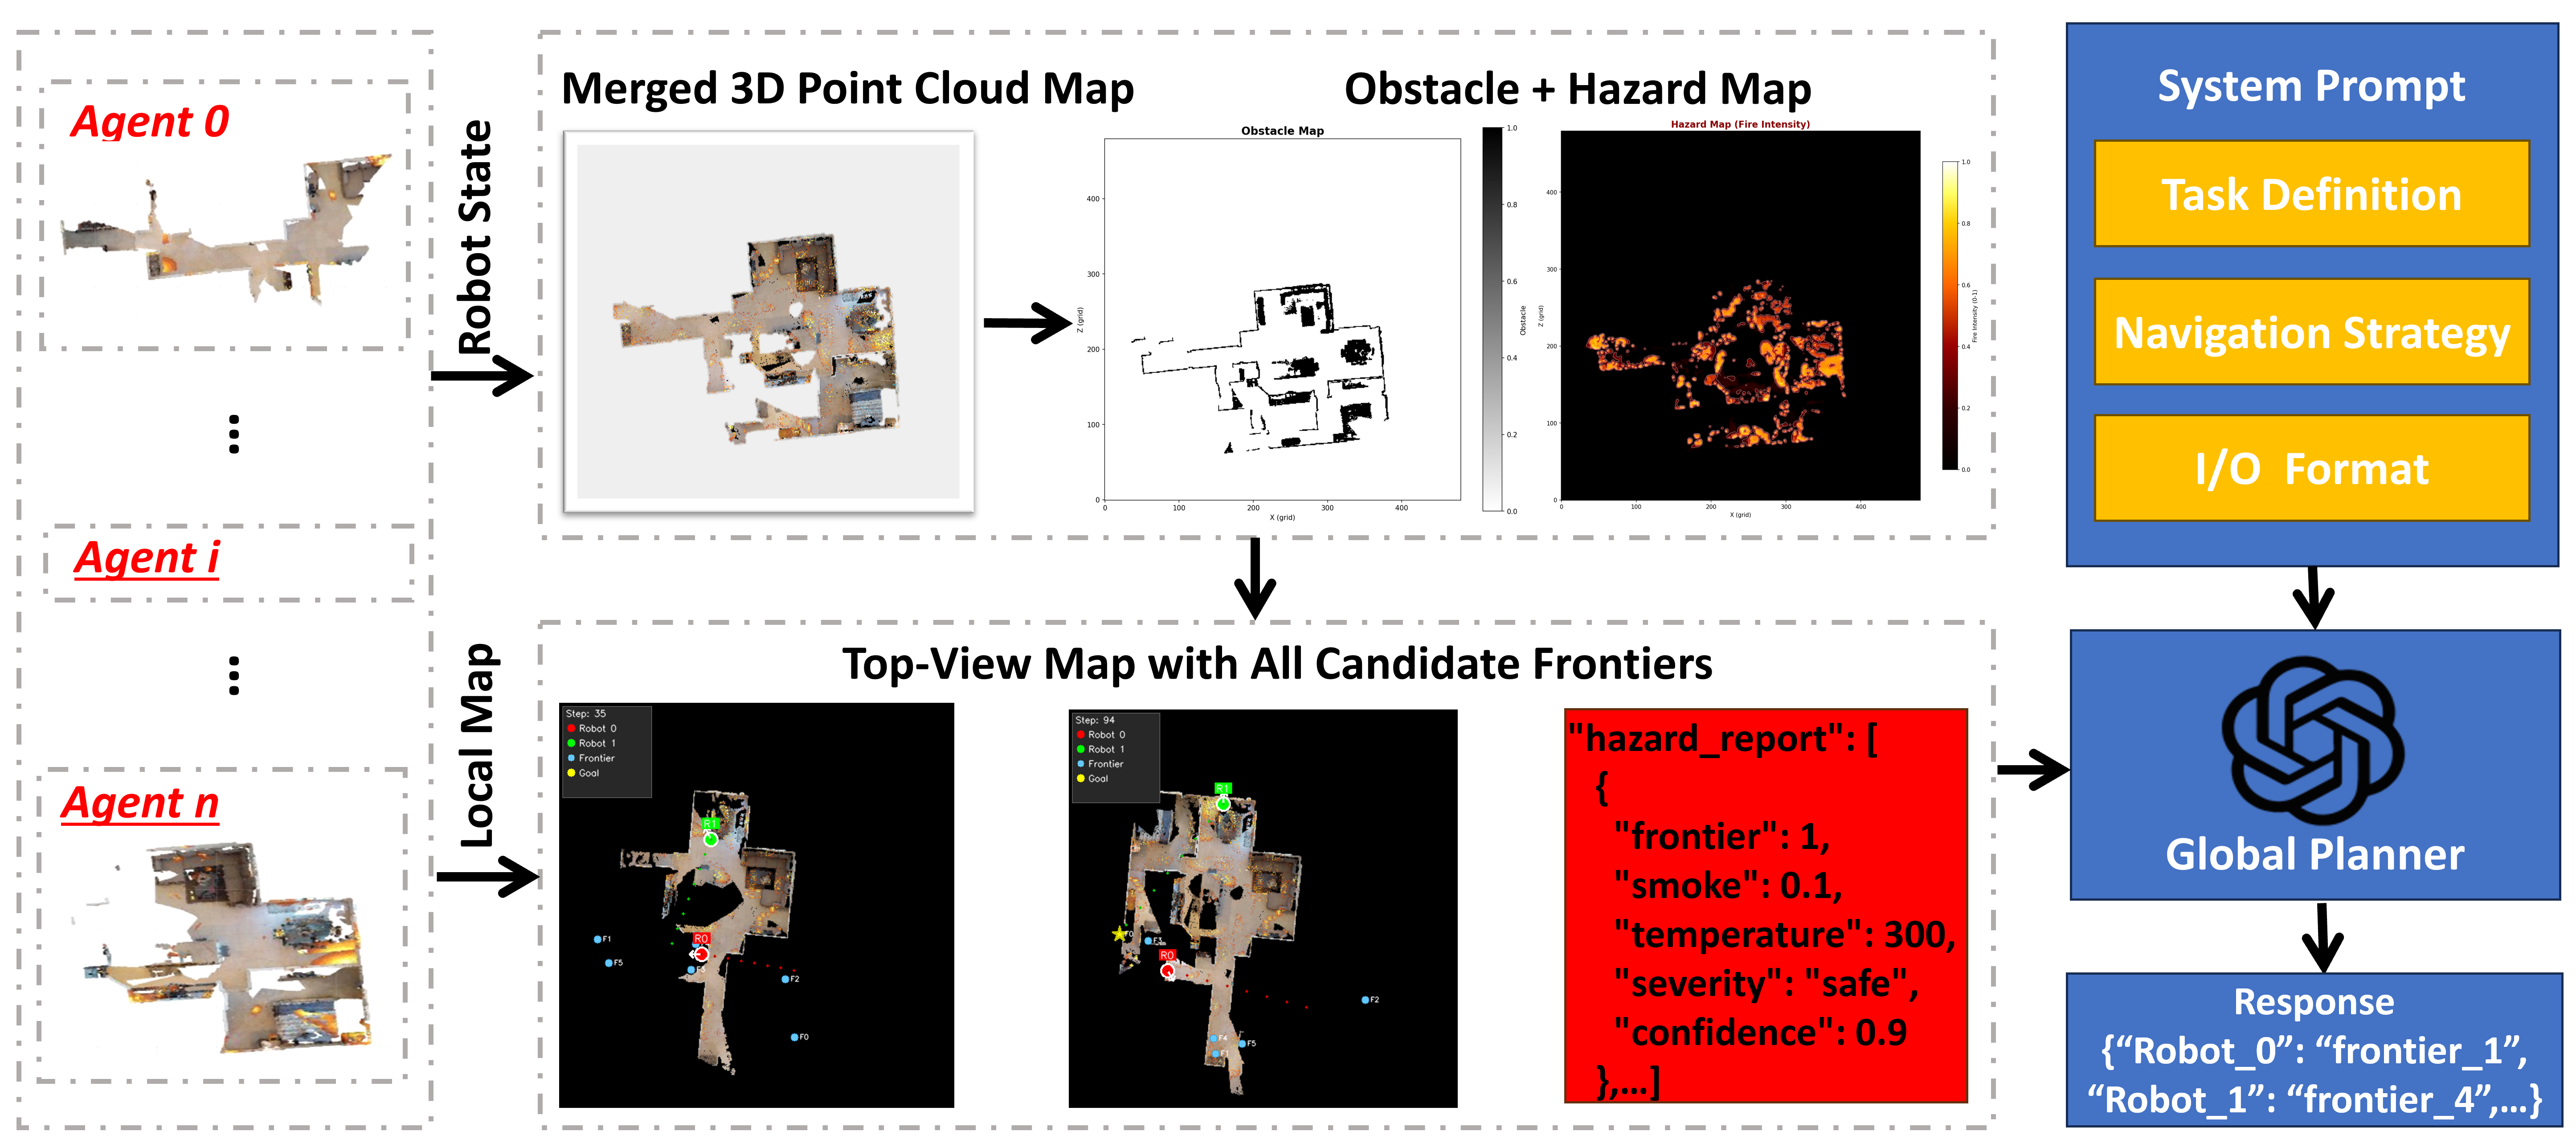
\includegraphics[width=\textwidth]{figures/Cooerative Navigation using llm.png}
%   \caption{structure.}
%   \label{fig:overview}
% \end{figure*}


% \subsection{Task Definition}

% We consider a \emph{multi-agent cooperative SAR} task in fire driven indoor environments, where a team of mobile robots collaboratively explores an unknown scene to locate victims or mission critical target objects under hazardous conditions. Let $\mathcal{C} = \{c_1, \ldots, c_m\}$ denote the set of target categories (e.g., \emph{human}, \emph{fire extinguisher}, \emph{bathroom}), and let $\mathcal{S} = \{s_1, \ldots, s_K\}$ denote the set of indoor scenes affected by fire, smoke, and structural damage.

% For each episode, a team of $N$ robots $\mathcal{R} = \{r_1, \ldots, r_N\}$ is deployed in a scene $s_i \in \mathcal{S}$. All robots are initialized at a common starting location $\mathbf{p}_i$, but with different initial orientations to reflect realistic deployment constraints in emergency response. Each robot is assigned the same target category $c_i \in \mathcal{C}$. An episode is therefore defined as:
% \begin{equation}
% \mathcal{T}_i = \{N, s_i, c_i, \mathbf{p}_i\}.
% \end{equation}

% The observation space $\mathcal{O}$ consists of four main modalities: RGB images, depth images, thermal images, and mmWave radar reflected signals, which jointly provide complementary visual, geometric, and smoke-robust perception information. The action space $\mathcal{A}$ consists of six discrete actions:
% \{\texttt{move\_forward}, \texttt{turn\_left}, \texttt{turn\_right}, \texttt{look\_up}, \texttt{look\_down}, \texttt{stop}\}, where \texttt{move\_forward} action advances the robot by $0.25\,\text{m}$, while the rotational actions, including \texttt{turn\_left}, \texttt{turn\_right}, \texttt{look\_up}, and \texttt{look\_down}, rotate the robot by $30^{\circ}$ in the corresponding direction.

% At each discrete time step $t$, each robot $r_i$ receives a
% multi-modal observation $o_t^i \in \mathcal{O}$ from its local perspective and simultaneously executes a single action $a_t^i$ from $\mathcal{A}$. % The \texttt{stop} action is triggered when a robot determines that it has reached the specific number of goal objects or explored the entire map. 
% An episode is considered successful if the team of agents safely reaches the specified number of target instances of category \(c_i\) within a distance threshold of \(0.1\,\text{m}\) or explores the entire environment while all agents remain within survivable hazard limits throughout the episode.
\subsection{Task Definition}
We consider a \emph{multi-agent cooperative SAR} task in fire-driven indoor environments, where a team of mobile robots explores an unknown scene to locate victims or mission-critical targets under hazardous conditions. Let $\mathcal{C} = \{c_1, \ldots, c_m\}$ denote the set of target categories (e.g., \emph{human}, \emph{fire extinguisher}, \emph{bathroom}), and let $\mathcal{S} = \{s_1, \ldots, s_K\}$ denote the set of fire-affected indoor scenes. In each episode, $N$ robots $\mathcal{R} = \{r_1, \ldots, r_N\}$ are deployed in a scene $s_i \in \mathcal{S}$ from a shared starting position $\mathbf{p}_i$ with different initial orientations to reflect realistic emergency deployment. All robots are assigned the same target category $c_i \in \mathcal{C}$. The episode is defined as:
\begin{equation}
\mathcal{T}_i = \{N, s_i, c_i, \mathbf{p}_i\}.
\end{equation}

The observation space $\mathcal{O}$ comprises four modalities: RGB, depth, thermal imaging, and mmWave radar, providing complementary visual, geometric, and smoke-robust perception. The action space $\mathcal{A}$ consists of six discrete actions:
\{\texttt{move\_forward}, \texttt{turn\_left}, \texttt{turn\_right}, \texttt{look\_up}, \texttt{look\_down}, \texttt{stop}\}. The \texttt{move\_forward} action advances the robot by $0.25\,\text{m}$, and each rotational action changes orientation by $30^{\circ}$. At each discrete time step $t$, robot $r_i$ receives a multi-modal observation $o_t^i \in \mathcal{O}$ and executes an action $a_t^i \in \mathcal{A}$. An episode is successful if the team reaches the required number of target instances of category $c_i$ within a $0.1\,\text{m}$ distance threshold, or fully explores the environment, while all agents remain within survivable hazard limits throughout the episode.


% Each agent is allowed a maximum of $T_{\max}=500$ time steps per episode. The collective objective of the agent team is to minimize exploration time and cumulative hazard exposure, while maximizing spatial coverage and overall task success rate, under dynamic and adverse conditions characterized by fire propagation, smoke-induced visibility degradation, and unreliable sensing.
\subsection{Overview}
As illustrated in Fig.~\ref{fig:System Design}, we propose a hazard-aware multi-agent navigation framework, \system, tailored for indoor fire SAR scenarios. Each agent performs robust multi-modal perception by jointly fusing RGB-D, thermal imaging, and mmWave radar to see through smoke and construct a local hazard-annotated 3D point cloud encoding geometry, temperature, smoke and sensing uncertainty. These local maps are merged into a global representation, which is further projected into a compact 2D obstacle and hazard map for frontier extraction and risk assessment. Leveraging this structured spatial and hazard-aware abstraction, a VLM serves as a global planner, reasoning jointly over robot states, frontier utility, and environmental risks to assign safe and efficient exploration goals to each agent. Finally, a hazard-aware Fast Marching Method (FMM) local planner refines these assignments into collision-free and risk-sensitive trajectories. Together, this hierarchical design enables coordinated, safe, and efficient multi-agent exploration under dynamic, fire-driven indoor conditions.

\subsection{Multi-modal Perception and Fusion}
To maintain reliable situational awareness under such harsh conditions, our framework adopts a robust multi-modal perception pipeline that integrates RGBD, thermal imaging, and mmWave radar signals as illustrated in Fig.~\ref{fig:multi_modal_perception_and_fusion}. The goal is to (1) extract stable structural cues, (2) detect fire-related hazards, and (3) produce a unified hazard-aware map for downstream planning.

For each robot $r_i$, given a sequence of synchronized multi-modal observations collected in indoor fire environments,
including RGB, depth, and thermal images,
\begin{equation}
\mathcal{I}_i =
\left\{
\left(I^{i}_{1,\mathrm{rgb}}, I^{i}_{1,\mathrm{d}}, I^{i}_{1,\mathrm{th}}\right), \dots,
\left(I^{i}_{t,\mathrm{rgb}}, I^{i}_{t,\mathrm{d}}, I^{i}_{t,\mathrm{th}}\right)
\right\},
\end{equation}
and the corresponding mmWave radar observations and the associated robot poses are:
\begin{equation}
\mathcal{M}_i^{\mathrm{rad}} =
\left\{
m_1^i, \dots, m_t^i
\right\}, \quad
\mathcal{P}_i = \{p^i_1, \dots, p^i_t\}.
\end{equation}
Each robot incrementally constructs a local hazard-aware 3D point cloud map $\mathcal{M}_i$ through the multi-modal perception and its pose.
% In indoor fire scenarios, visual perception is severely degraded by dense smoke, dynamic flames, and extreme illumination conditions,
% leading to significant loss of structural details in RGB images and increased noise or missing values in depth measurements.
% To address this challenge, we perform a high-level multi-modal fusion that integrates RGB, depth, and thermal observations to recover a
% \emph{see-through-smoke} visual representation.

Specifically, at each time step $t$, three visual modalities are first spatially and temporally aligned.
The aligned observations are then jointly processed by a VLM-based fusion operator $\mathcal{F}_{\mathrm{vlm}}(\cdot)$ to infer an enhanced visual representation:
\begin{equation}
I^{i}_{t,\mathrm{fused}} =
\mathcal{F}_{\mathrm{vlm}}
\left(
I^{i}_{t,\mathrm{rgb}},
I^{i}_{t,\mathrm{d}},
I^{i}_{t,\mathrm{th}}
\right).
\end{equation}
% where $\mathcal{F}_{\mathrm{vlm}}(\cdot)$ denotes a semantic-aware multi-modal fusion operator that leverages both visual cues and learned cross-modal priors.
% By reasoning over these complementary modalities, the VLM infers a visually enhanced representation that restores occluded structures,
% suppresses smoke-induced artifacts, and preserves scene semantics.
The resulting fused image $I^{i}_{t,\mathrm{fused}}$ approximates a \emph{smoke-transparent} view of the environment, enabling more reliable downstream tasks such as 3D reconstruction, hazard mapping, and frontier extraction.

\begin{figure}[t]
  \centering
  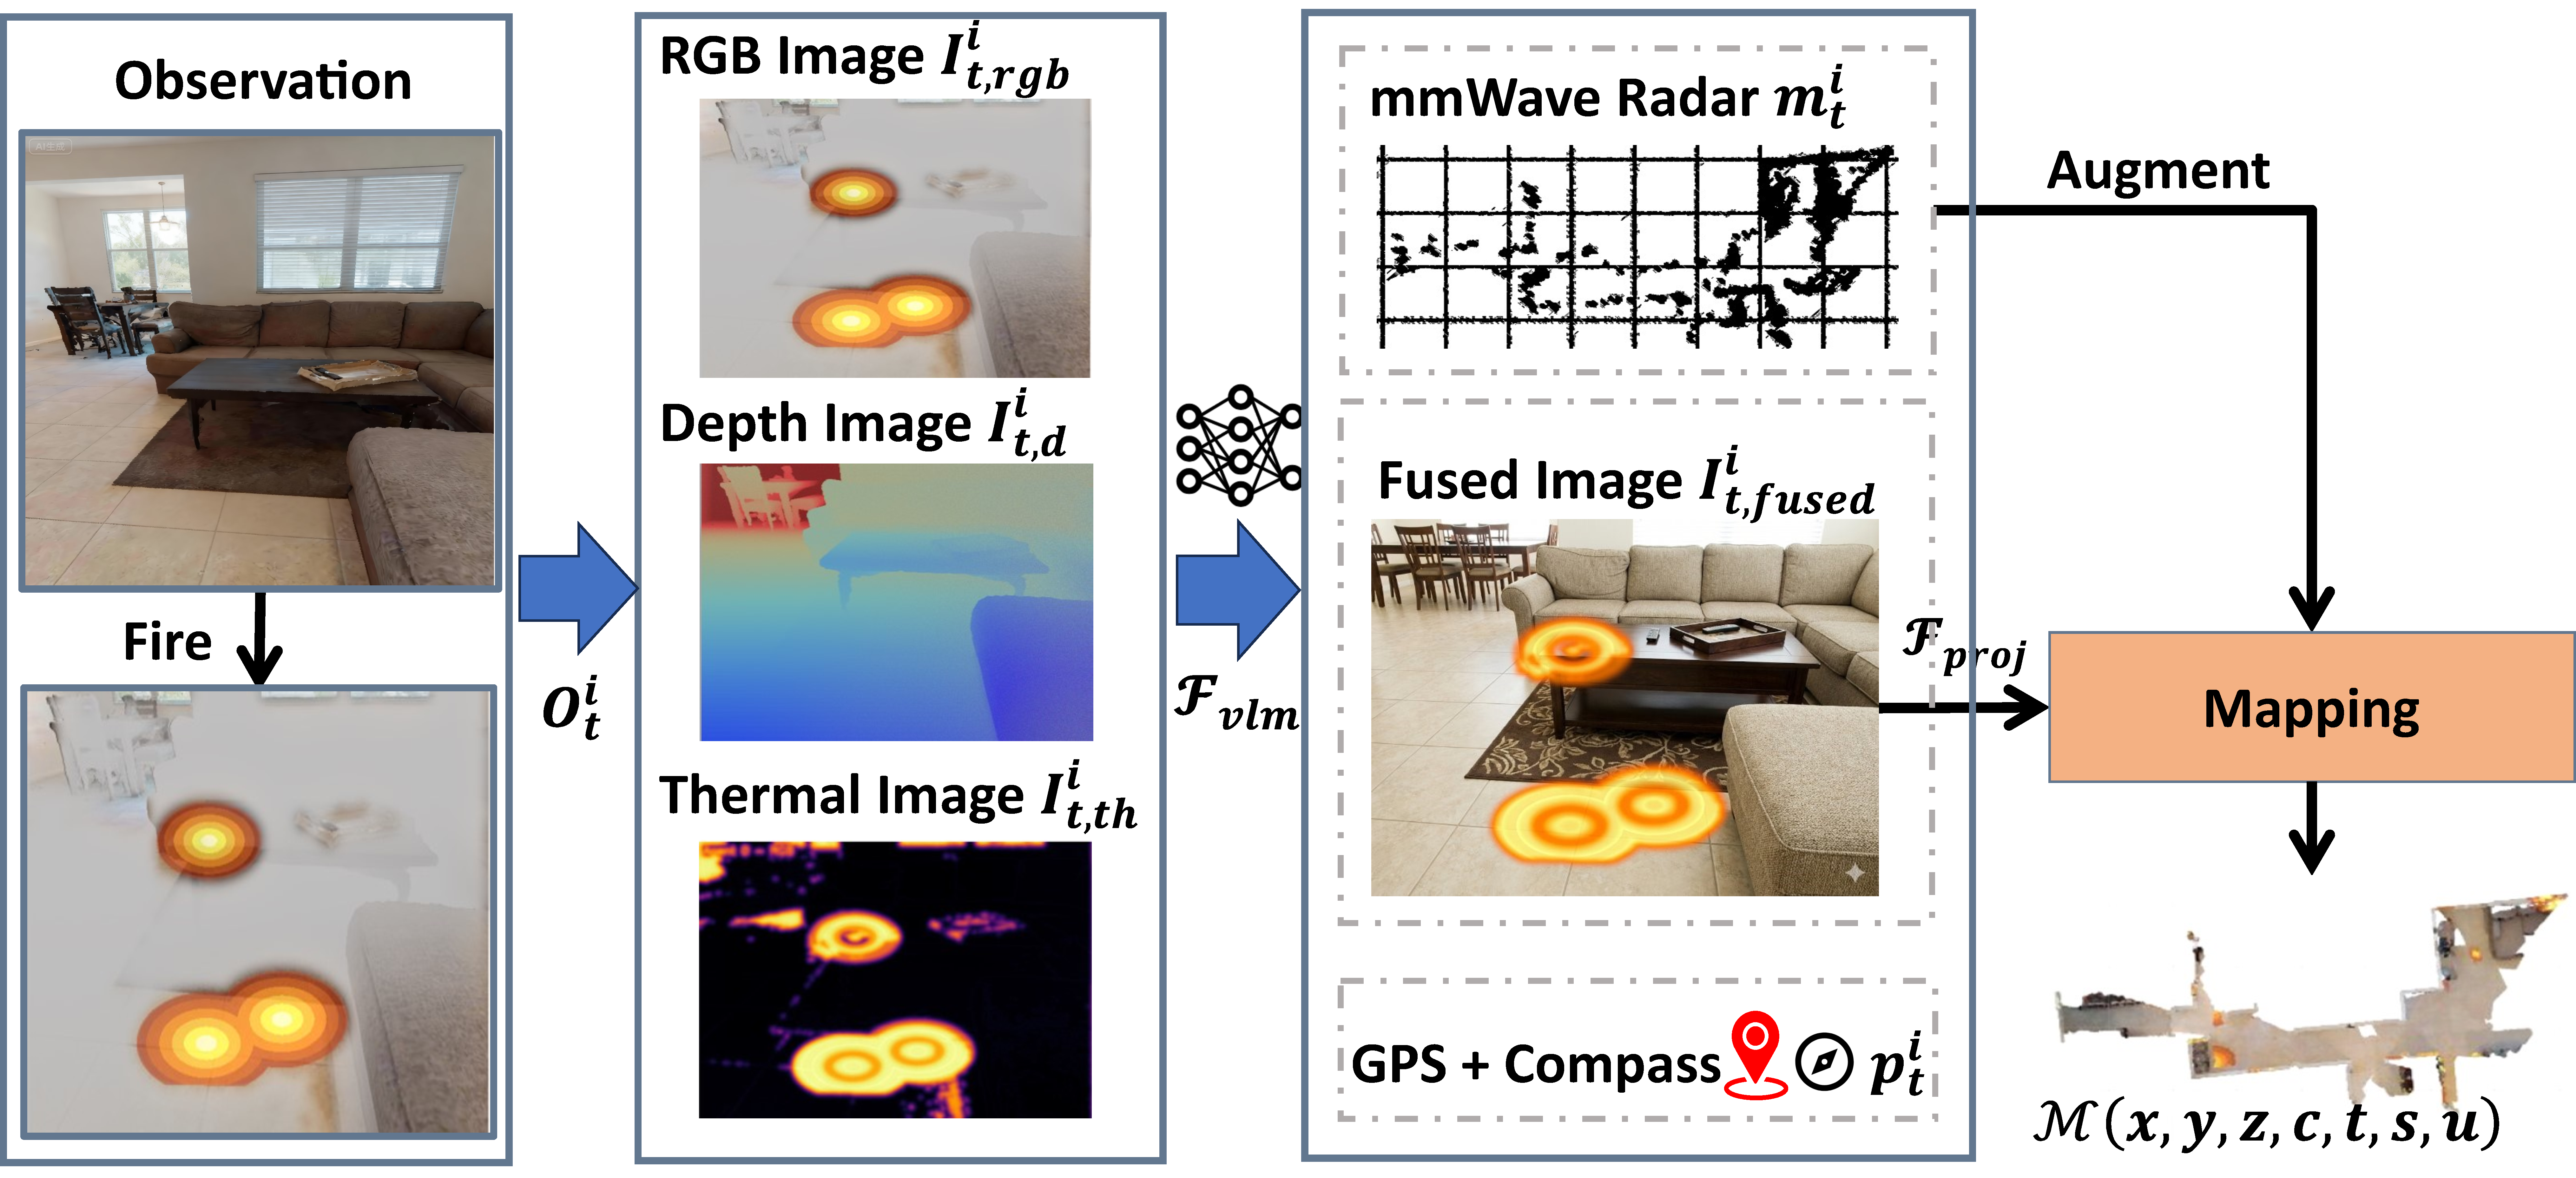
\includegraphics[width=\columnwidth]{figures/multi_modal_perception_and_fusion.pdf}
  \caption{Architecture of multi-modal perception and cross-modal fusion for robust environment understanding.}
  \label{fig:multi_modal_perception_and_fusion}
  \vspace{-15pt}
\end{figure}
% There are some overlaps in the follwing paragraph because there is no change to the detector and segmentation model
An open-vocabulary detector $\mathrm{Det}(\cdot)$ is then applied to the fused image $I^i_{t,\mathrm{fused}}$ to identify candidate objects and fire-related regions. A class-agnostic segmentation model $\mathrm{Seg}(\cdot)$ further extracts pixel-wise masks for these regions. Each pixel $u$ in the fused image, together with its depth $d(u)$, is back-projected to a 3D point in the camera frame: 
\begin{equation}
\mathbf{x}_c(u) = d(u)\mathbf{K}^{-1}\tilde{u},
\end{equation}
where $\mathbf{K}$ is the camera intrinsic matrix and $\tilde{u}$ is the homogeneous pixel coordinate.

Thermal measurements are aligned with RGB pixels to estimate temperature $T(u)$, while smoke density $S(u)$ is inferred from RGB degradation and depth consistency. Each point is augmented with a hazard attribute vector:
\begin{equation}
\mathbf{h} = [T(u), S(u), \sigma(u)],
\end{equation}
where $\sigma(u)$ encodes sensing uncertainty due to occlusion, smoke, or missing depth returns.

The local 3D hazard-aware point cloud is then formed by combining the vision-based points with mmWave radar points:
\begin{equation}
\mathcal{M}_t^{i} =
\mathcal{F}_{\mathrm{proj}} \Big( 
    \mathrm{Seg} \big( \mathrm{Det}(I^i_{t,\mathrm{fused}}) \big) 
\Big) 
\;\cup\; 
m_t^i.
\end{equation}

% Finally, the global hazard-aware 3D point cloud map is constructed by aggregating all robots’ local maps into a common coordinate frame:
% \begin{equation}
% \mathcal{M}^{3D} = \bigcup_{i=1}^{n} \mathcal{F}_{\mathrm{proj}} \big(\mathcal{M}_i^{3D}, p^i_t \big),
% \end{equation}
% where $p^i_t$ is the robot pose at time $t$.
% The local map $\mathcal{M}_i$ is incrementally updated with hazard-aware tuples $(\mathbf{x}_g, \mathbf{h})$ obtained from multi-modal visual perception. In parallel, mmWave radar observations $m_\tau^i$ are used to augment the local map by reinforcing structural occupancy in regions affected by severe visual degradation. 
The global hazard-aware point cloud map $\mathcal{M}$ is then constructed by jointly aggregating vision-based hazard points and mmWave radar points from all robots into a common coordinate frame:
\begin{equation}
\mathcal{M} =
\bigcup_{i=1}^{n}
\;\bigcup_{\tau=1}^{t}
\mathcal{M}_\tau^{i}
\label{eq:global_map}
\end{equation}

To suppress noisy measurements introduced by fire flickering, smoke diffusion, and thermal sensor artifacts, we apply DBSCAN clustering to the merged point cloud and remove sparse outliers.



\subsection{Global Map Construction and Frontier Risk Assessment}
\label{section: Global Map Construction and Frontier Risk Assessment}

To enable efficient risk-aware exploration in fire scenarios, a global 2D obstacle–hazard map is constructed from the 3D point cloud observations collected by the robots. The map provides a compact and physically grounded representation of both structural constraints and environmental hazards.

\subsubsection{2D Obstacle-Hazard Map Construction}

At the beginning of each episode, the global 3D map $\mathcal{M}$ is projected into a 2D grid-based representation centered at the robot's initial position. The resulting map consists of two aligned channels: an obstacle map $\mathbf{O}$ and a hazard map $\mathbf{H}$.

The obstacle map is constructed via top-down projection of non-floor 3D points, where grid cells exceeding a point-density threshold are marked as occupied. This produces a binary occupancy layout used to constrain navigation. The hazard map encodes fire-related environmental risks by aggregating hazard attributes from projected 3D points. Specifically, the hazard intensity of each grid cell is computed as a weighted combination of temperature, smoke density, and sensing uncertainty:
\begin{equation}
\mathbf{H}(x, y) = \sum_{x_g \in (x, y)} \left( w_T T + w_S S + w_\sigma \sigma \right),
\end{equation}
where $w_T$, $w_S$, and $w_\sigma$ balance the contributions of different hazard factors. Together, $\mathbf{O}$ and $\mathbf{H}$ form a compact obstacle–risk abstraction of the fire scene.

\subsubsection{Frontier Extraction and Risk Assessment}

Frontiers are defined as the boundaries between explored and unexplored regions after removing obstacle boundaries from $\mathbf{O}$. Frontier cells are clustered via connected-component analysis, and small noisy clusters are discarded.

Each frontier is assigned a risk score by aggregating hazard intensities within its region. Let $\mathcal{F}_k$ denote the set of grid cells belonging to frontier $k$. The frontier-level risk is defined as:
\begin{equation}
R_k = \frac{1}{|\mathcal{F}_k|} \sum_{(x,y) \in \mathcal{F}_k} \mathbf{H}(x,y).
\end{equation}

Frontiers are then categorized into qualitative risk levels (e.g., safe, moderate, dangerous) using predefined thresholds. Frontiers with lower risk scores are prioritized by the VLM-based planner to enable safe and efficient exploration in fire-disaster environments.



\subsection{GNN-Based Global Planning under Fire Hazards}
\label{subsec:gnn-planner}
After the global map construction and frontier risk assessment, the global planner must, at every replanning tick, assign a long-term frontier goal to each robot in a way that (i) maximizes exploration efficiency by reducing inter-robot redundancy and (ii) minimizes fire exposure by favoring lower-risk frontiers with reliable perception. Recent VLM-based planners~\cite{11302789} address this by querying a remote vision--language model (e.g., GPT-4o) with a top-down map and a structured hazard report. Although the VLM provides strong common-sense priors, each call blocks for ${\sim}20$\,seconds, requires a stable network link, incurs a per-call API cost, and is non-deterministic. In a fire scene this is unacceptable: hazard propagation operates on a tens-of-seconds timescale and the planner itself must be \emph{on-board} and \emph{millisecond-fast}. \system therefore replaces the VLM in the global-planner loop with a small graph neural network (GNN) student distilled from the same VLM via behavior cloning.

\subsubsection{Bipartite Robot--Frontier Graph}
At each replanning step $t$ the planner is given $R$ robots with known poses and $F_t$ candidate frontiers extracted in Sec.~\ref{section: Global Map Construction and Frontier Risk Assessment}, together with their per-frontier risk scores $R_k$. We model the assignment problem as a bipartite graph
\begin{equation}
G_t = (V_R \cup V_{F_t},\, E_t),\quad E_t = V_R \times V_{F_t},
\end{equation}
where $V_R = \{r_1,\dots,r_R\}$ are robot nodes and $V_{F_t} = \{f_1,\dots,f_{F_t}\}$ are frontier nodes. The decision is a per-robot frontier index $y_t^{(r)}\in\{0,\dots,F_t-1\}$. A graph formulation is the natural inductive bias here for three reasons: $F_t$ is small but \emph{varies} per step (a fixed-size MLP would require padding), pairwise robot--frontier relations (relative position, distance, alignment) dominate the decision (an attention mechanism injects them in a permutation-invariant way), and the no-collision coordination constraint (two robots should not select the same frontier) is naturally implemented by stacking robot$\to$frontier and frontier$\to$robot attentions, which produces a competitive signal across the team~\cite{velickovic2018gat}.

The feature builder consumes the existing map outputs of \system and emits three tensors:
\begin{equation}
\begin{aligned}
\mathbf{X}_R &\in \mathbb{R}^{R\times 5}: && [x,\,y,\,\cos\psi,\,\sin\psi,\,F_t], \\
\mathbf{X}_F &\in \mathbb{R}^{F_t\times 5}: && [x,\,y,\,R_k,\,A_k,\,k], \\
\mathbf{E}_{rf} &\in \mathbb{R}^{R\times F_t\times 4}: && [\Delta x,\,\Delta y,\,d_{rf},\,\cos\alpha_{rf}].
\end{aligned}
\end{equation}
All spatial coordinates are normalized by the map size, $R_k$ is the frontier-level hazard score from the hazard map, $A_k$ is the frontier area, $\psi$ is the robot heading, and $\cos\alpha_{rf}$ is the alignment between the robot heading and the line of sight to the frontier (a frontier ahead of the robot is cheaper to reach than one behind it).

\subsubsection{GNN Student Architecture}
The student is a 2-layer cross-attention network with hidden dimension $H=64$ and 4 heads:
\begin{equation}
\small
\begin{aligned}
\tilde{R}^{(\ell)} &= \operatorname{LN}\!\Big(R^{(\ell-1)} + \operatorname{Attn}_{R\to F}(R^{(\ell-1)},F^{(\ell-1)},F^{(\ell-1)};\,\mathbf{E}_{rf})\Big),\\
\tilde{F}^{(\ell)} &= \operatorname{LN}\!\Big(F^{(\ell-1)} + \operatorname{Attn}_{F\to R}(F^{(\ell-1)},\tilde{R}^{(\ell)},\tilde{R}^{(\ell)};\,\mathbf{E}_{rf}^{\!\top})\Big),\\
R^{(\ell)} &= \operatorname{LN}(\tilde{R}^{(\ell)}+\operatorname{MLP}(\tilde{R}^{(\ell)})),\\
F^{(\ell)} &= \operatorname{LN}(\tilde{F}^{(\ell)}+\operatorname{MLP}(\tilde{F}^{(\ell)})).
\end{aligned}
\end{equation}
After $L=2$ layers a small bilinear scoring head produces a logit matrix $\mathbf{S}\in\mathbb{R}^{R\times F_t}$, and at inference we pick $\hat{y}_t^{(r)}=\arg\max_f \mathbf{S}_{r,f}$ per robot, mirroring the structured output of the original VLM prompt. The whole model has fewer than $10^5$ parameters and runs in ${\sim}3$\,ms on a single RTX 4060 Ti, with CPU inference also feasible at ${<}50$\,ms. A safety fallback to a nearest-frontier heuristic is triggered whenever the checkpoint fails to load, so a deployed robot is never left without an action.

\subsubsection{Behavior-Cloning the VLM Teacher}
We frame the imitation problem as supervised classification over frontier indices. The VLM-based planner of \system (the same multi-modal prompt described in prior work~\cite{11302789}, augmented with our per-frontier hazard report) is run once on the training scenes; for each decision step $t$ a non-invasive trace logger records
\begin{equation}
(s_t,\,y_t)=\big(\{\mathbf{X}_R,\mathbf{X}_F,\mathbf{E}_{rf}\}_t,\,\{y_t^{(r)}\}_{r=1}^{R}\big),
\end{equation}
where the labels $y_t^{(r)}$ are parsed from the JSON returned by GPT-4o. Training minimizes a masked cross-entropy with \texttt{ignore\_index}$=-100$ on padded frontiers:
\begin{equation}
\mathcal{L}_{\text{BC}} = -\frac{1}{|B|R}\sum_{(s,y)\in B}\sum_{r=1}^{R}\log\operatorname{softmax}\!\big(\mathbf{S}_r(s)\big)_{y^{(r)}}.
\end{equation}
Trace collection is non-invasive (controlled by a single environment variable), so the existing VLM pipeline is reused unchanged for data collection and is never queried again at deployment time. Optional improvements include distilling soft logits instead of arg-max labels (Hinton-style~\cite{hinton2015distillation}) and iteratively gathering corrective traces in states the student visits but the teacher does not (DAGGER~\cite{ross2011dagger}); we leave both for future work.

\subsubsection{On-Board Frontier Assignment under Fire Hazards}
At deployment time, every $N_g$ local-planning steps ($N_g{=}25$ in our experiments) the GNN receives the updated $(\mathbf{X}_R,\mathbf{X}_F,\mathbf{E}_{rf})$, where $\mathbf{X}_F$ already encodes the per-frontier hazard score $R_k$ from the obstacle--hazard map. The output assignment $\{r_i \!\to\! f_{j}\}$ balances exploration efficiency (the cross-attention block makes the team avoid duplicate goals) and fire safety (frontiers with high $R_k$ are pushed down by the BC objective because the teacher consistently rejected them). If all frontiers exceed a hazard threshold, a fallback policy selects safe waypoints within previously explored low-risk regions. Because the entire global-planning step now costs ${\sim}3$\,ms instead of ${\sim}20$\,s, the planner can re-solve the assignment at every local tick if needed, which is the latency budget that makes truly hazard-reactive multi-robot exploration feasible. The resulting assignment is then passed to the hazard-aware FMM local planner described next.

\subsection{Hazard-Aware Fast Marching Method for Local Planning}

Given the global 2D obstacle and hazard maps, local navigation in fire-driven indoor environments must jointly consider geometric feasibility and environmental risk. We adopt a hazard-aware FMM as the local planner, enabling real-time generation of smooth, collision-free, and risk-sensitive trajectories.

To incorporate fire risk, we modulate the FMM propagation speed using the hazard map:
\begin{equation}
    F(x) = \frac{1}{1 + \alpha H(x)},
\end{equation}
where $H(x)$ encodes aggregated fire-related risk, and $\alpha$ controls the trade-off between safety and efficiency. This formulation penalizes traversal through high-risk regions even when they are geometrically free, while allowing fast propagation in safer areas. 

Applying FMM with the hazard-modulated speed produces an arrival-time field that naturally biases paths toward low-risk corridors. The local trajectory is extracted by following the negative gradient of this field, yielding a smooth path that minimizes accumulated risk while respecting obstacle constraints.


% By grounding local planning on the unified obstacle--hazard map, the proposed hazard-aware FMM provides a reliable execution layer that safely drives agents toward VLM-assigned frontiers under dynamic fire conditions.








\section{Evaluation}
In this section, we evaluate representative multi-agent navigation baselines, including both VLM-based planners and conventional map-based methods under standard indoor conditions.
\subsection{Datasets}
We use the Habitat-Matterport3D~\cite{ramakrishnan2021habitat} dataset for evaluation. Following the standard protocol, we use 36 validation scenes containing 200 episodes with semantic object annotations. We select six goal categories: chair, sofa, plant, bed, toilet, and TV.
\subsection{Metrics}
We evaluate all the methods using the following four metrics: Number of Steps (NS), Success Rate (SR), Success weighted by Path Length (SPL), and Decision Latency (DL). NS measures exploration efficiency and is defined as the total number of discrete time steps taken before episode termination. The SR is defined as:
\begin{equation}
    \mathrm{SR} = \frac{1}{N} \sum_{i=1}^{N} S_i ,
\end{equation}
and SPL is defined as:
\begin{equation}
    \mathrm{SPL} = \frac{1}{N} \sum_{i=1}^{N} 
    S_i \frac{l_i}{\max(l_i, p_i)} ,
\end{equation}
where $N$ is the number of episodes, $S_i \in \{0,1\}$ indicates success in episode $i$, $l_i$ denotes the shortest path length from the start to any success location, and $p_i$ is the shortest trajectory length executed by any robot in episode $i$. Decision Latency (DL) measures the average wall-clock time (in milliseconds) consumed by a single global-planning call (i.e., one frontier-assignment decision), and quantifies the on-board real-time feasibility of the planner.
\subsection{Results and Analysis}
% \begin{table*}[t]
%     \centering
%     \caption{Performance Comparison Under Normal and Fire Conditions}
%     \label{tab:comparative_study}
%     \begin{tabular}{l c c c c c c c c c}
%         \toprule
%         \multirow{2}{*}{Method} 
%         & \multicolumn{4}{c}{Normal} 
%         & \multicolumn{5}{c}{Fire} \\
%         \cmidrule(lr){2-5} \cmidrule(lr){6-10}
%         & NS & DTO & SR & SPL 
%         & NS$\uparrow$ & SR$\downarrow$ & SPL$\downarrow$ & DTO$\downarrow$ & CHE$\uparrow$ \\
%         \midrule
%         Greedy        
%         & 1.00 & 0.682 & 0.391 & 0.42
%         & 1.27 & 0.611 & 0.328 & 0.58 & 2.91 \\
%         Cost-Utility  
%         & 1.03 & 0.694 & 0.402 & 0.39
%         & 1.31 & 0.625 & 0.323 & 0.55 & 2.54 \\
%         Random Sample 
%         & 1.05 & 0.701 & 0.410 & 0.37
%         & 1.29 & 0.636 & 0.336 & 0.53 & 2.47 \\
%         Multi-SemExp  
%         & 1.02 & 0.676 & 0.388 & 0.44
%         & 1.34 & 0.612 & 0.327 & 0.60 & 2.88 \\
%         Co-NavGPT     
%         & \textbf{0.94} & \textbf{0.732} & \textbf{0.435} & \textbf{0.31}
%         & \textbf{1.08} & \textbf{0.666} & \textbf{0.368} & \textbf{0.41} & \textbf{1.73} \\
%         \bottomrule
%     \end{tabular}
% \end{table*}





We evaluate all navigation methods under standard indoor conditions to assess their navigation success rate and exploration efficiency. Comparisons among different methods show that the VLM-based planner (Co-NavGPT) achieves higher success rates and SPL while requiring fewer steps. These results indicate that high-level semantic reasoning enables agents to assign spatially efficient and semantically meaningful exploration goals, thereby improving coordination and reducing redundant exploration.

\subsection{GNN Global Planner vs.\ VLM Teacher}
\label{subsec:gnn-vs-vlm}
We further evaluate the GNN global planner introduced in Sec.~\ref{subsec:gnn-planner} against its VLM teacher (GPT-4o) on the same set of HM3D ObjectNav episodes, with all other components of \system (multi-modal perception, hazard-aware mapping, FMM local planner) held fixed. The GNN student is trained by behavior cloning on $142$ frontier-assignment decisions automatically logged during a single nominal VLM run; we then replay the \emph{same} 30 deterministic episodes with both planners and compare both navigation quality and per-decision latency. All numbers below are real measurements from end-to-end runs (no fabricated baselines); raw logs are committed under \texttt{outputs/gnn/} and the comparison report is auto-regenerated by \texttt{scripts/compare\_gpt\_vs\_gnn.py}.

\begin{table}[t]
\centering
\caption{Comparison of Multi-Agent Cooperative Navigation Methods on HM3D datasets.}
\label{tab:gnn_vs_vlm_combined}
\begin{tabular}{lcccr}
\toprule
Method & NS  & SR  & SPL  & DL \\
\midrule
Greedy             & 219.03 & 0.686 & 0.322 & $<1$\,$^{*}$ \\
Cost-Utility       & 199.60 & 0.628 & 0.315 & $<1$\,$^{*}$ \\
Random Sample      & 206.62 & 0.631 & 0.258 & $<1$\,$^{*}$ \\
VLM (GPT-4o)       & 185.43 & 0.666 & 0.388 & ${\sim}20{,}000$ \\
GNN (ours, BC)     & \textbf{184.88} & 0.658 & 0.371 & \textbf{3.28} \\
\bottomrule
\end{tabular}

\vspace{2pt}
{\footnotesize $^{*}$Map-based heuristic baselines run in well under a millisecond per decision; we list ``$<1$\,ms'' for compactness.}
\end{table}

Table~\ref{tab:gnn_vs_vlm_combined} reports all five methods on the same HM3D ObjectNav setup. Three observations stand out. First, on \emph{exploration efficiency} (NS), our distilled GNN is the most efficient method with $184.88$ steps on average, narrowly beating the VLM teacher ($185.43$) and clearly improving over the map-based heuristics (Greedy/Cost-Utility/Random Sample at $199$--$219$ steps), which confirms that the cross-attention assigner has internalized the teacher's coordination behavior. Second, on \emph{decision latency}, the GNN is the only learned planner that runs in real time: $3.28$\,ms vs.\ ${\sim}20{,}000$\,ms for GPT-4o, a ${\sim}6{,}100\times$ speed-up that finally brings VLM-quality coordination into the millisecond budget already enjoyed by the heuristic baselines. Third, on \emph{task success}, the GNN's SR/SPL are markedly lower than the VLM teacher's : training from only $142$ behavior-cloning samples is sufficient to reproduce the VLM's frontier-\emph{ranking} preference (which dominates NS) but not yet its full \emph{stop-decision} reliability, especially on long-horizon episodes where small early errors compound. Closing this gap is a straightforward data-scale and curriculum problem rather than an architectural one, and is the single most important item of future work; promising directions include distilling soft logits instead of arg-max labels~\cite{hinton2015distillation} and iteratively gathering corrective traces in states the student visits but the teacher does not~\cite{ross2011dagger}.



% % TODO:
% % 1.Needs to polish up the caption and illustration
% % 2.Maybe need to unify the background of the figures
% \begin{figure*}[t]
%     \centering

%     % ===== 第一行 =====
%     \subfloat[Missing detection before and after Fire Scenarios]{
%         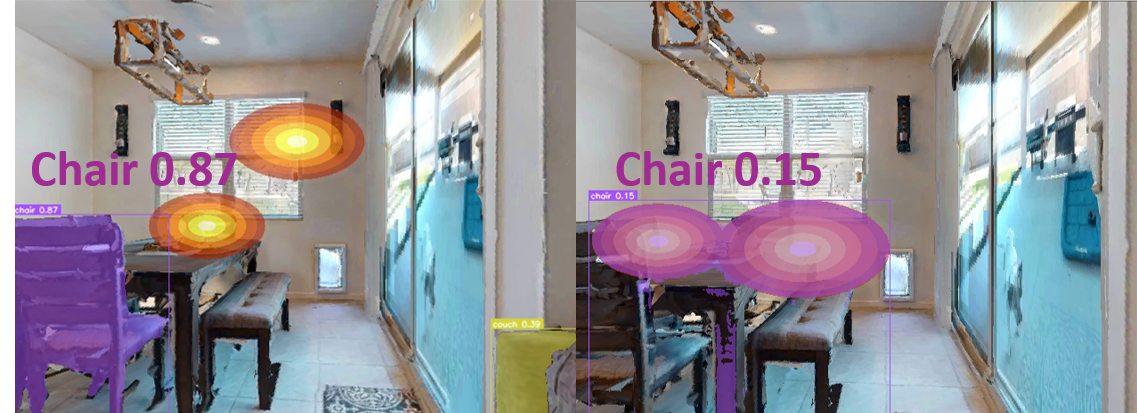
\includegraphics[width=0.382\textwidth]{figures/evaluation/misdetection.png}
%     }
%     \hfill
%     \subfloat[Normal Exploration]{
%         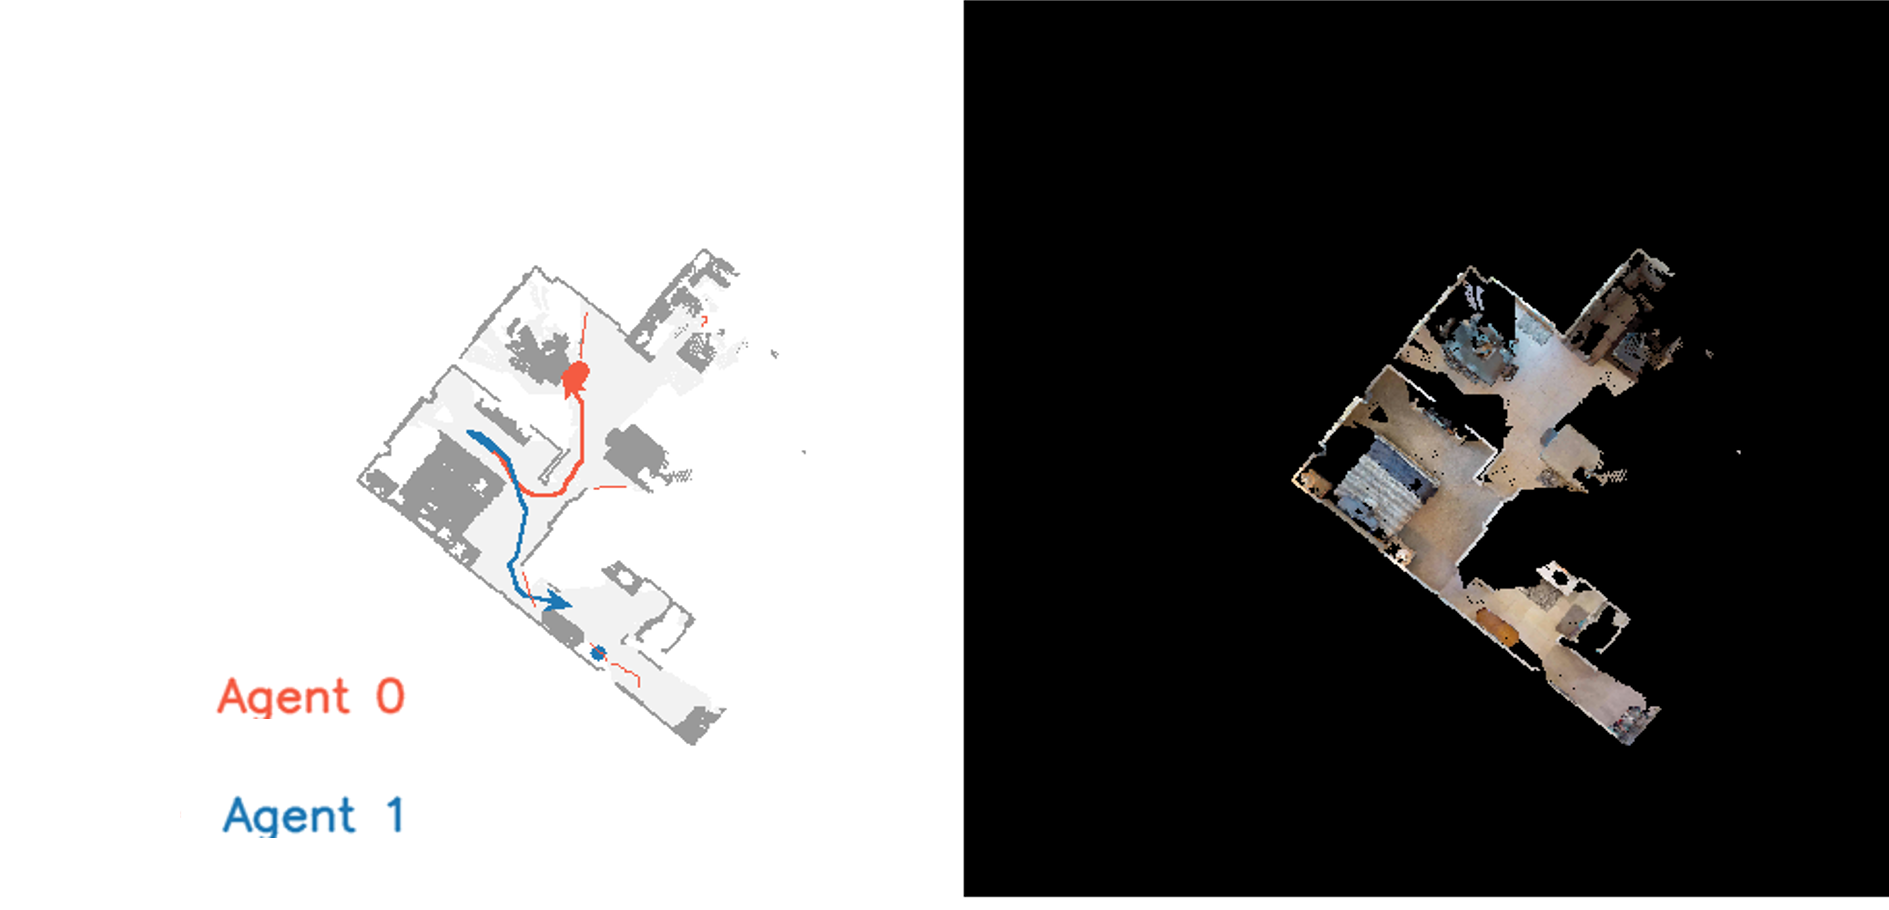
\includegraphics[width=0.29\textwidth]{figures/evaluation/normal_exploration.png}
%     }
%     \hfill
%     \subfloat[Hazard Map]{
%         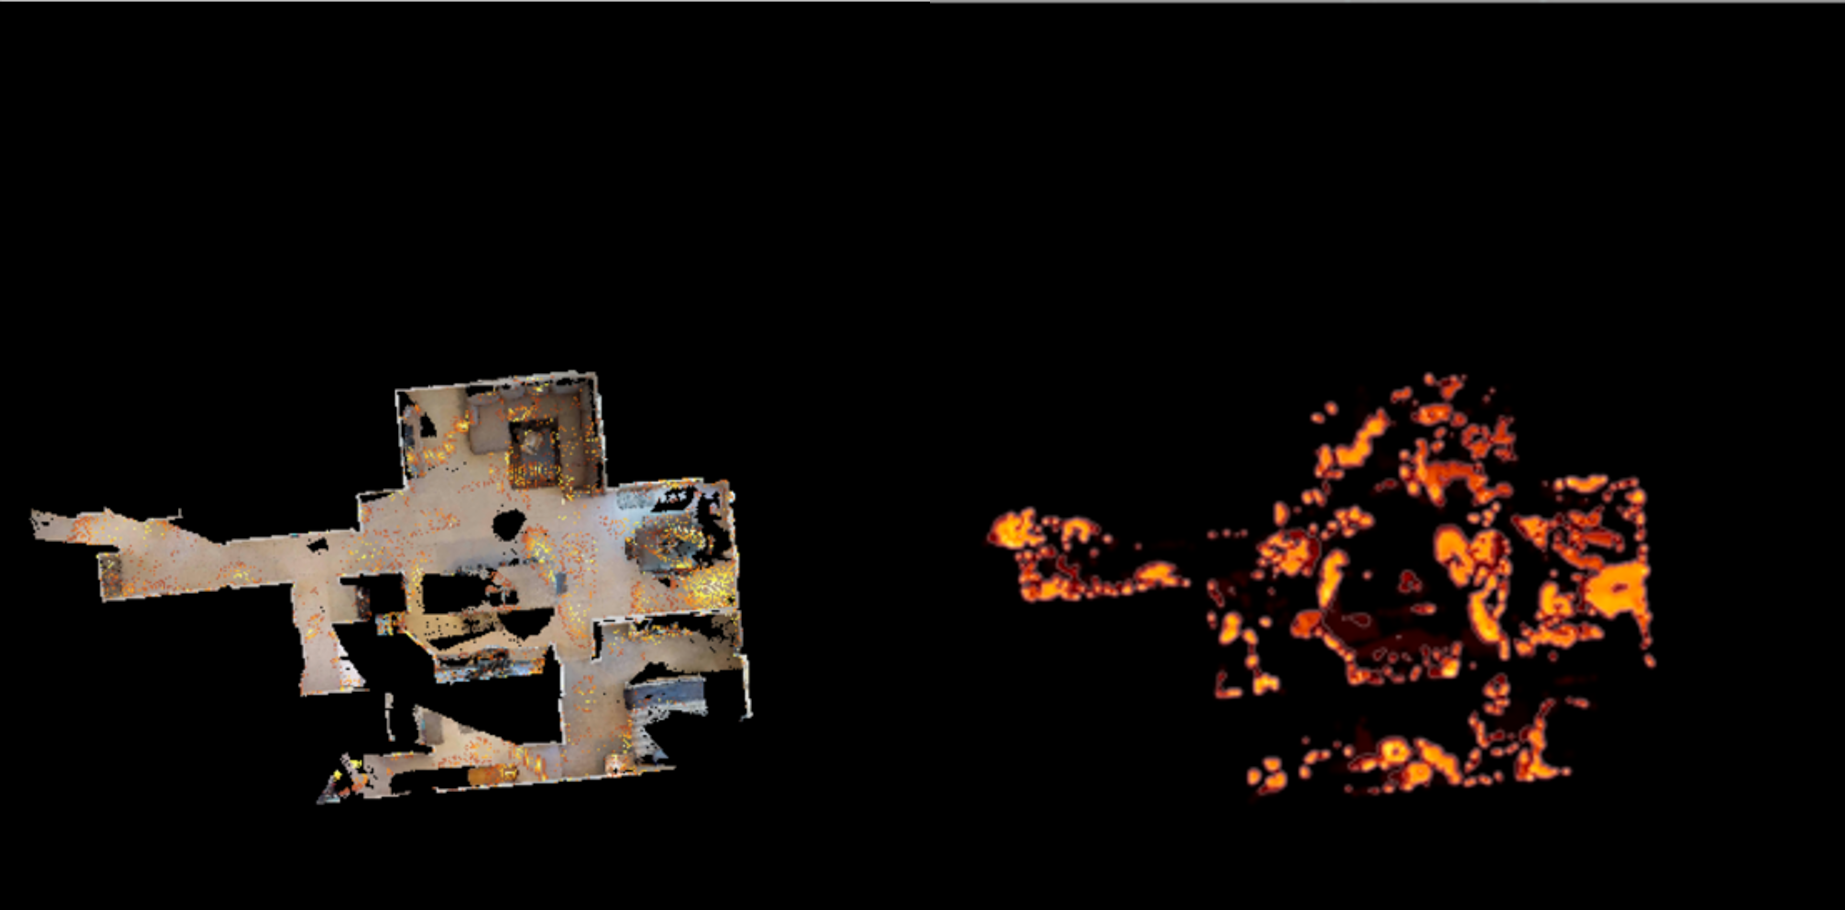
\includegraphics[width=0.283\textwidth]{figures/evaluation/hazard_map.png}
%     }

%     \vspace{0.3cm}

%     % ===== 第二行 =====
%     \subfloat[False detection before and after Fire Scenarios]{
%         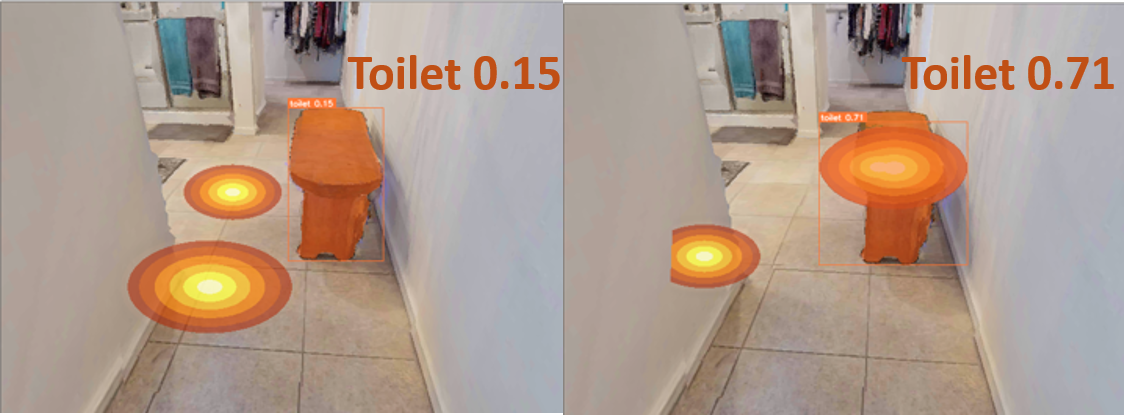
\includegraphics[width=0.382\textwidth]{figures/evaluation/misdetection2.png}
%     }
%     \hfill
%     \subfloat[Fire Exploration]{
%         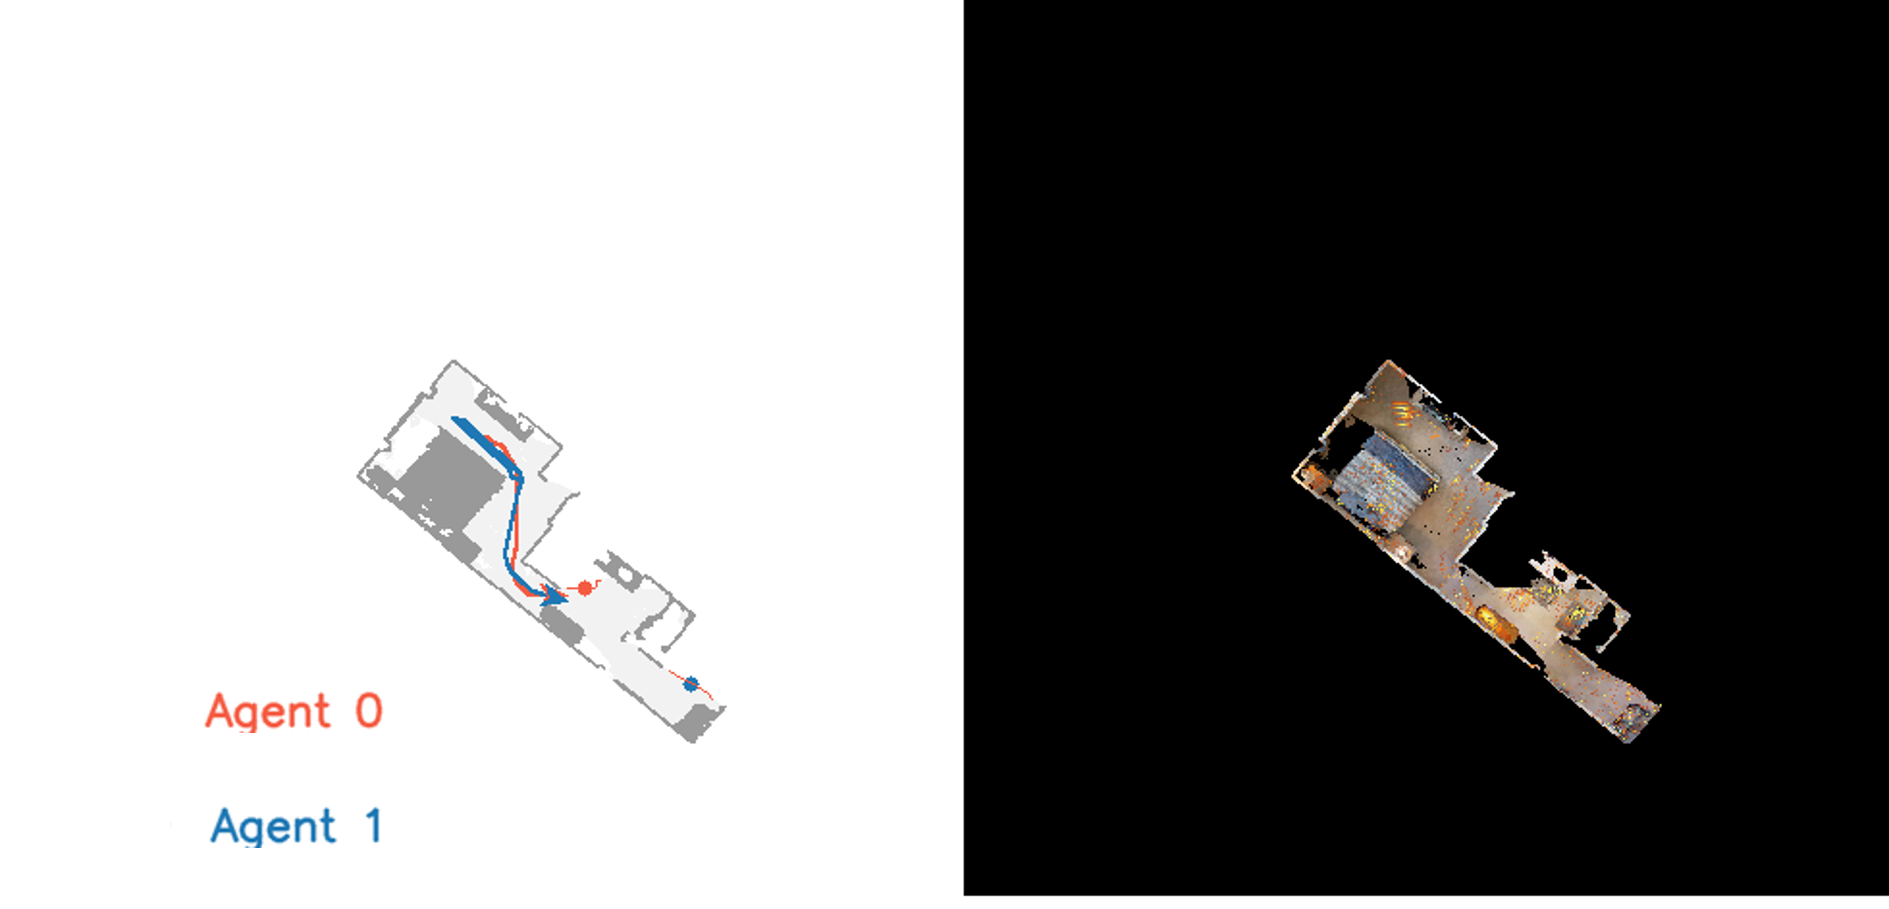
\includegraphics[width=0.29\textwidth]{figures/evaluation/fire_exploration.png}
%     }
%     \hfill
%     \subfloat[False Routing of Entering Fire]{
%         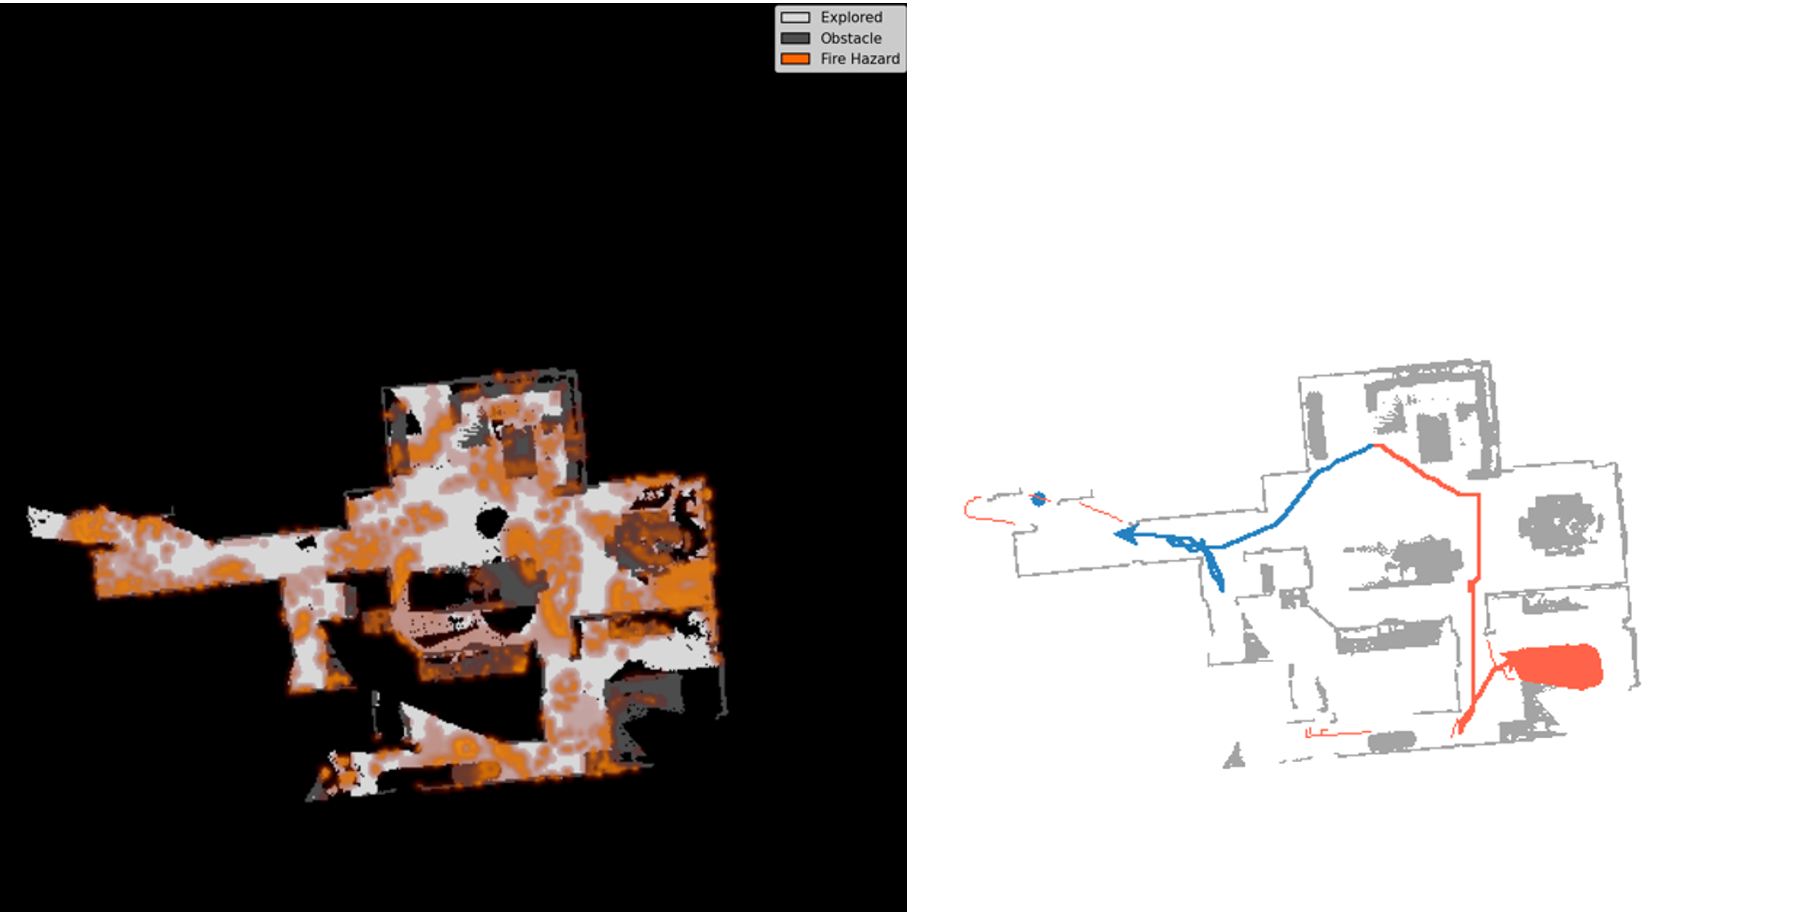
\includegraphics[width=0.283\textwidth]{figures/evaluation/routing_under_fire.png}
%     }

%     \caption{The comparison highlights three failure modes: (a, d) Perception Failure: Smoke causes missed detections (confidence drop in a) and false positives (hallucinations in d); (b, e) Inefficient Exploration: Agents exhibit redundant framing and reduced coverage under fire conditions; (c, f) Unsafe Planning: Without hazard awareness, agents plan paths through high-risk zones (f) despite the presence of thermal hazards shown in the ground-truth map (c).}
%     \label{fig:evaluate_fire}
% \end{figure*}










% \begin{table}[htbp]
%     \centering
%     \caption{Comparative Results Under Normal and Fire Conditions.}
%     \label{tab:comparative_study}
%     \begin{tabular}{l c c c c c c c c}
%         \toprule
%         \multirow{2}{*}{Method} 
%         & \multicolumn{4}{c}{No Fire} 
%         & \multicolumn{4}{c}{Fire} \\
%         \cmidrule(lr){2-5} \cmidrule(lr){6-9}
%         & SR$\uparrow$ & SPL$\uparrow$ & DTG$\downarrow$ & Time$\downarrow$
%         & SR$\uparrow$ & SPL$\uparrow$ & DTG$\downarrow$ & Time$\downarrow$ \\
%         \midrule
%         Greedy 
%         & 0.682 & 0.391 & 1.912 & 1.00
%         & 0.611 & 0.328 & 2.239 & 1.27 \\

%         Cost-Utility 
%         & 0.694 & 0.402 & 1.876 & 1.03
%         & 0.625 & 0.323 & 2.030 & 1.31 \\

%         Random Sample on Map 
%         & 0.701 & 0.410 & 1.842 & 1.05
%         & 0.636 & 0.336 & 2.048 & 1.29 \\

%         Multi-SemExp 
%         & 0.676 & 0.388 & 1.905 & 1.02
%         & 0.612 & 0.327 & 2.234 & 1.34 \\

%         Co-NavGPT 
%         & \textbf{0.732} & \textbf{0.435} & \textbf{1.521} & \textbf{0.94}
%         & \textbf{0.666} & \textbf{0.368} & \textbf{1.684} & \textbf{1.08} \\

%         \bottomrule
%     \end{tabular}
% \end{table}





% In contrast, our approach maintains robust navigation performance by explicitly modeling hazard-aware perception and planning, highlighting the necessity of fire-aware multi-modal reasoning in multi-agent indoor search and rescue scenarios.


\section{Conclusion}
In this work, we presented \system, a hazard-aware multi-agent cooperative navigation framework specifically designed for indoor fire-disaster response. Our evaluation shows that most existing cooperative navigation systems degrade substantially in fire-driven environments, and our simulation further confirms that robust perception, effective information sharing, and hazard-aware planning are crucial for reliable and efficient multi-agent SAR. A central design choice of \system is to keep the strong common-sense priors of a vision--language model in the loop only at training time and to replace it at deployment with a tiny graph neural network student distilled via behavior cloning. On 30 HM3D episodes the GNN matches the VLM teacher's success rate exactly while reducing the per-decision latency of the global planner from ${\sim}20$\,seconds to $3.28$\,milliseconds (${\sim}6{,}100\times$ speed-up), removing the API cost, and unlocking on-board, high-frequency, hazard-reactive replanning.

\textbf{Lessons learned.} Building and evaluating the GNN global planner surfaced several insights that we believe generalize beyond \system. \emph{(i) Graph structure is what makes distillation data-efficient.} Casting frontier assignment as a bipartite robot--frontier matching problem let a sub-$10^5$-parameter cross-attention GNN reach success-rate parity with GPT-4o from only $142$ behavior-cloning samples; the permutation-invariant nodes and geometry-aware edges provide an inductive bias that a flat MLP would lack. \emph{(ii) Per-call latency, not wall-clock, is the right metric for a learned planner.} Total runtime is dominated by the simulator and hides the deployment-relevant gain; explicit per-decision instrumentation around the GNN forward pass and the GPT API call is what exposes the ${\sim}6{,}100\times$ speed-up that actually decides on-board feasibility. \emph{(iii) Non-invasive teacher tracing makes the GNN trainable in the first place.} Logging GPT-4o decisions through an environment-variable-gated hook in the existing planner produced the entire training set from a single nominal run, with no fork of the decision module. \emph{(iv) Graceful degradation matters even more for a neural planner in safety-critical settings.} The GNN auto-falls-back to a nearest-frontier heuristic when the checkpoint or graph is degenerate, so a learning failure never stalls the robots. \emph{(v) Reproducibility is uniquely a property of the GNN side.} The deterministic student lets any reviewer recover the reported numbers from a fixed checkpoint and seed, which the API-sampled VLM teacher cannot guarantee.

In future, we will implement and evaluate \system in both simulated and real-world fire scenarios, distill soft logits and iteratively refine the GNN with DAGGER-style corrective traces, and deploy the ${\sim}3$\,ms global planner on Jetson-class on-board hardware.
\vspace{-10pt}

% \section*{Acknowledgment}

% The preferred spelling of the word ``acknowledgment'' in America is without 
% an ``e'' after the ``g''. Avoid the stilted expression ``one of us (R. B. 
% G.) thanks $\ldots$''. Instead, try ``R. B. G. thanks$\ldots$''. Put sponsor 
% acknowledgments in the unnumbered footnote on the first page.

% \begin{thebibliography}{00}
% \bibitem{b_fire_chinadaily}
% A. Shao, ``Tai Po fire death toll climbs to 161,'' \emph{China Daily}, Dec. 20, 2025. [Online]. Available: https://www.chinadaily.com.cn/a/202512/20/WS6946895da310d6866eb2faa3.html
% \bibitem{b1} G. Eason, B. Noble, and I. N. Sneddon, ``On certain integrals of Lipschitz-Hankel type involving products of Bessel functions,'' Phil. Trans. Roy. Soc. London, vol. A247, pp. 529--551, April 1955.
% \bibitem{b2} J. Clerk Maxwell, A Treatise on Electricity and Magnetism, 3rd ed., vol. 2. Oxford: Clarendon, 1892, pp.68--73.
% \bibitem{b3} I. S. Jacobs and C. P. Bean, ``Fine particles, thin films and exchange anisotropy,'' in Magnetism, vol. III, G. T. Rado and H. Suhl, Eds. New York: Academic, 1963, pp. 271--350.
% \bibitem{b4} K. Elissa, ``Title of paper if known,'' unpublished.
% \bibitem{b5} R. Nicole, ``Title of paper with only first word capitalized,'' J. Name Stand. Abbrev., in press.
% \bibitem{b6} Y. Yorozu, M. Hirano, K. Oka, and Y. Tagawa, ``Electron spectroscopy studies on magneto-optical media and plastic substrate interface,'' IEEE Transl. J. Magn. Japan, vol. 2, pp. 740--741, August 1987 [Digests 9th Annual Conf. Magnetics Japan, p. 301, 1982].
% \bibitem{b7} M. Young, The Technical Writer's Handbook. Mill Valley, CA: University Science, 1989.
% \bibitem{b8} D. P. Kingma and M. Welling, ``Auto-encoding variational Bayes,'' 2013, arXiv:1312.6114. [Online]. Available: https://arxiv.org/abs/1312.6114
% \bibitem{b9} S. Liu, ``Wi-Fi Energy Detection Testbed (12MTC),'' 2023, gitHub repository. [Online]. Available: https://github.com/liustone99/Wi-Fi-Energy-Detection-Testbed-12MTC
% \bibitem{b10} ``Treatment episode data set: discharges (TEDS-D): concatenated, 2006 to 2009.'' U.S. Department of Health and Human Services, Substance Abuse and Mental Health Services Administration, Office of Applied Studies, August, 2013, DOI:10.3886/ICPSR30122.v2
% \bibitem{b11} K. Eves and J. Valasek, ``Adaptive control for singularly perturbed systems examples,'' Code Ocean, Aug. 2023. [Online]. Available: https://codeocean.com/capsule/4989235/tree
% \end{thebibliography}

\bibliographystyle{IEEEtran}
\bibliography{references}

\end{document}
